\section{YOLO9000 (YOLOv2)}  \label{sec:yolov2}

YOLO9000, also known as YOLOv2, is an improvement of the YOLOv1 model \cite{yolo9000_2017}. The real-time object detection model YOLOv2 was first introduced in 2016. The name YOLO9000 stems from the fact that the model is capable of detecting over 9,000 object categories in real time,  which is significantly more than the original YOLO model. This is achieved by finetuning the model with the WordNet language database, which also is the database that the ImageNet labels set pulls from.

\subsection{Accuracy Improvement}
The YOLOv2 model proposes five changes that improve the accuracy of YOLOv1. The first change is the addition of \textbf{batch normalization} on the convolutional layer, which improves the YOLOv1 mAP score by more than 2\%. Batch normalization removes the need for dropout technique \cite{dropout_2014}, which drops certain activated neurons to avoid overfitting problem \cite{szeliski_cv_book}. The second change is utilizing \textbf{higher resolution classifier}. While YOLOv1 only trains on $224 \times 224$ images for the classification task, YOLOv2 further trains the classifier with $448 \times 448$ images. The higher resolution classifier increases the YOLOv1 mAP score by 4\%. The third change is the use of \textbf{passthrough layer}. Since the convolutional layer decreases the image's spatial dimension gradually, thus it becomes more difficult to detect smaller objects in the image as more convolutional layers are used. For this reason, the passthrough layer help brings the image detail from the higher spatial dimension to the lower spatial dimension map, similar to the skip connection in ResNet \cite{resnet_2016}.

Since each divided cell in YOLOv1 only predicts exactly 2 bounding boxes, 1 confidence score, and 1 classification label (the highest probability class), thus the model has poor performance in detecting objects that appear near together, especially small objects. To address this problem, the YOLOv2 model proposes the fourth and fifth changes. 

The fourth change is utilizing \textbf{anchor boxes} at each cell instead of randomly initializing the bounding box like in YOLOv1. The size and aspect ratio of the anchor box heavily depends on the domain that the model will be applied to. For example, when applying the model to the traffic detection task, then the main shape and size the model need to look for are pedestrian and different vehicle. Thus starting the anchor box at these shape and size improve the runtime for both training and inference. For this reason, a k-means clustering algorithm is used to find the top-k common dimension in the training set \cite{yolo9000_2017}. The anchor boxes are then used to predict the bounding box. The YOLOv2 model predicts five parameters for each bounding box $[t_x, t_y, t_w, t_h, and t_o]$, where $t_x, t_y$ and $t_w, t_h$ is the center and the dimension of the bounding box in relation to the cell and the image dimension, respectively. These five parameters are the same as the prediction made by YOLOv1. Given that the cell is $(c_x, x_y)$ offset from the top-left corner of the image, and the anchor box has the dimension of $p_w, p_h$, then the predicted bounding box has the center at $(b_x, b_y)$ with the dimension of $b_w, b_h$, and can be computed with constraint by sigmoid function, as shown in Figure \ref{fig:yolov2_bbox}.

\begin{figure}[!ht]
    \centering
    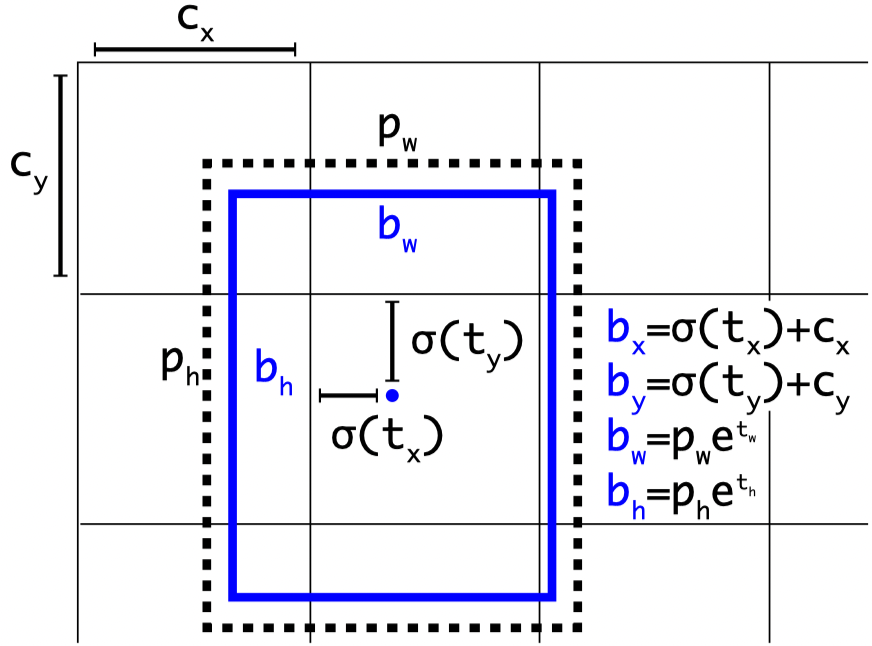
\includegraphics[width=3in]{figures/yolov2_bbox.png}
    \caption{YOLOv2 bounding box (in blue) generation offset from the anchor box (in black) \cite{yolo9000_2017}} 
    \label{fig:yolov2_bbox}
\end{figure}

Since the anchor boxes are used to predict the bounding box, this removes the need for fully connected layers. In addition to the removal of fully connected layers, the YOLOv2 model also moves the classification label from the cell level to the anchor box level. In other words, the YOLOv2 model predicts a classification label for each anchor box \cite{yolo9000_2017}. Let the image be divided into an $S \times S$ cell grid, each cell generates $B$ anchor boxes, and the dataset has $C$ categories, then the image detection is encoded as a $S \times S \times B*(4+1+C)$ tensor. The anchor box scheme removes the assumption of one object per grid cell and improves the mAP score by approximately 5\%.

The fifth change is \textbf{multi-scale training}. Since YOLOv2 remove the fully connected layer, thus it can process images of any size. Therefore, instead of training with a fixed size, the model chooses a new input image dimension every 10 batches. Additionally, since the model is downsampled by 32 times during its process, to avoid quantization, the input image should be a multiple of 32: {320, 352, ..., 608}. This training scheme forces the model to be able to predict object at different resolutions, which train the network to predict object of different scale. In addition to multi-scale training, the model also performs a data augmentation process, including crop, rotation, hue and saturation shift, and exposure shifts to expand the training dataset and further generalize the model.

\subsection{Runtime Improvement}
The YOLOv2 further simplifies the architecture used in YOLOv1. The YOLOv2 model uses a new classification model, namely Darknet-19. The overall architecture of Darknet-19 is shown in Figure \ref{fig:darknet19_archite}. Compared to the GoogLeNet, Darknet-19 is smaller, with 5.58 billion operations instead of 8.52 billion operations, while having higher top-5 accuracy in classification tasks after training \cite{yolo9000_2017}. Compared to YOLOv1's CNN architecture, Darknet-19 only has 19 convolutional layers and 5 max-pooling layers, while YOLOv1's CNN consists of 24 convolutional layers, 4 max-pooling layers, and 2 fully connected layers. The Darknet-19 is first trained with the ImageNet 1000 for the classification task. The Darknet-19 model is then adapted for the object detection task by replacing the last convolutional layer with three $3 \times 3$ convolutional layers that output 1024 channels, followed by $1 \times 1$ convolutional layer to convert $S \times S \times 1024$ to $S \times S \times B*(4+1+C)$.

\begin{figure}[!ht]
    \centering
    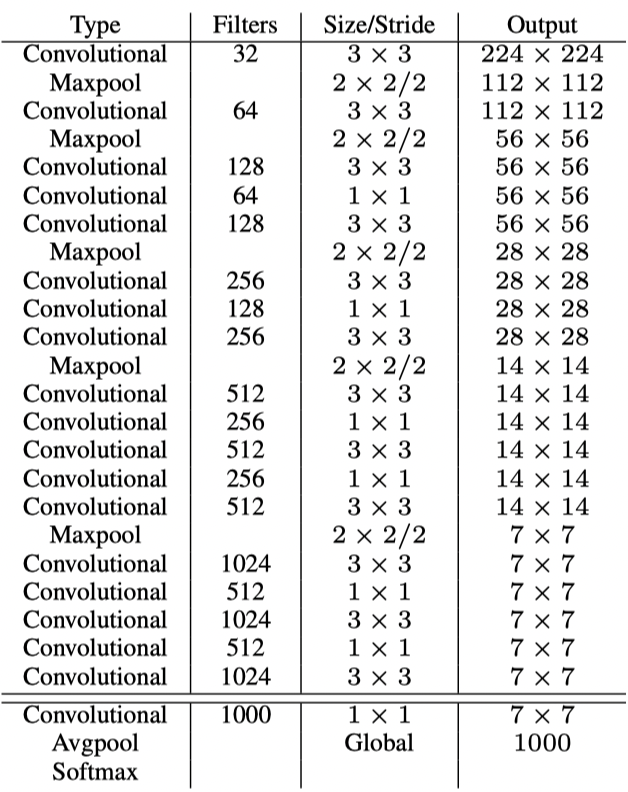
\includegraphics[width=4in]{figures/darknet19_archite.png}
    \caption{Darknet-19 architecture \cite{yolo9000_2017}} 
    \label{fig:darknet19_archite}
\end{figure}